\documentclass[a4j,11pt]{jarticle}
\usepackage{url}
\usepackage[dvipdfmx]{graphicx}
\usepackage[dvipdfmx]{color}
\usepackage[ipaex]{pxchfon}
\usepackage{listings}
\usepackage{plistings}
\usepackage{color}
\usepackage{amsmath, amssymb}
\usepackage{type1cm}


\definecolor{codegreen}{rgb}{0,0.6,0}
\definecolor{codegray}{rgb}{0.5,0.5,0.5}
\definecolor{codepurple}{rgb}{0.58,0,0.82}
\definecolor{backcolour}{rgb}{0.95,0.95,0.92}
 
\lstdefinestyle{mystyle}{
	language={c},
    backgroundcolor=\color{backcolour},   
    commentstyle=\color{codegreen},
    keywordstyle=\color{magenta},
    numberstyle=\tiny\color{codegray},
    stringstyle=\color{codepurple},
    basicstyle=\footnotesize,
    breakatwhitespace=false,         
    breaklines=true,                 
    captionpos=b,                    
    keepspaces=true,                 
    numbers=left,                    
    numbersep=5pt,                  
    showspaces=false,                
    showstringspaces=false,
    showtabs=false,                  
    tabsize=2
}
 
\lstset{style=mystyle}



\setlength{\textwidth}{1.1\textwidth}
\setlength{\oddsidemargin}{-3pt}
\setlength{\evensidemargin}{\oddsidemargin}
\setlength{\topmargin}{10mm}
\setlength{\headheight}{0mm}
\setlength{\headsep}{0mm}

\newcommand{\argmax}{\mathop{\rm argmax}\limits}
\newcommand{\argmin}{\mathop{\rm argmin}\limits}

\begin{document}

\begin{center}
%\noindent
 \vspace{10mm}

{\bf {\huge 先端機械学習 後半課題}}
%\end{center}

\vspace{80mm}

提出日:2021年 8月9日

\vspace{10mm}

情報工学系

\vspace{10mm}

学籍番号:18B14822

\vspace{10mm}


\vspace{20mm}

{\bf {\LARGE 宮崎 直哉}}
\end{center}





\newpage




\section{問題1}

\subsection*{パラメータbの値:}

\begin{equation*}
    b = (0, -1000, -1000, -2000, -2000, -3000)
\end{equation*}

\subsection*{パラメータbを求める方法:}
本問題では$w_i = 1000 (i = 1,2,3,4,5,6)$である。この時、シグモイド関数は下図のようになる。この時、このシグモイド関数はステップ関数と考えることができる。

\begin{figure}[hbtp]
    \centering
    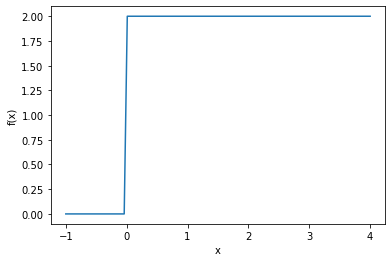
\includegraphics[width=10cm]{p1-3.png}
\end{figure}

この時、$g_i = v_i\sigma(1000x + b_i)$という式の意味を考えてみる。
すると、シグモイド関数はxから[0,1]区間への写像であるので、$v_i$はステップ関数の高さを表すことがわかる。また、
\begin{eqnarray*}
    g_i &=& v_i\sigma(1000x + b_i)\\
    &=& v_i\sigma\left( 1000(x + \frac{b_i}{1000}) \right))
\end{eqnarray*}
と変形すると、$x = -\frac{b_i}{1000}$がステップ関数の変換点となっていることがわかる。例えば、
\begin{equation*}
    f(x) = 
    \left\{
        \begin{array}{ll}
            0 & (x < 3) \\
            5 & (3 \leq x)
        \end{array}
    \right.
\end{equation*}
となるようなステップ関数をシグモイド関数で近似することを考えると、変換点が$x = -\frac{b_i}{1000} = 3$で高さ$v_i=5で$あるので、

\begin{equation*}
    g = 5\sigma(1000x - 3000)
\end{equation*}

とすれば、下図のようにステップ関数をシグモイド関数で近似したグラフを意図して得られる。
\begin{figure}[hbtp]
    \centering
    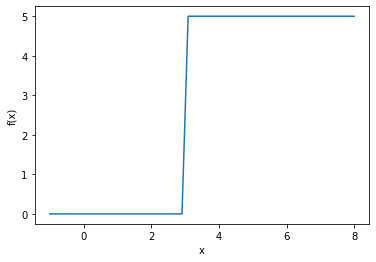
\includegraphics[width=10cm]{p1-4.png}
\end{figure}

\newpage

この性質を利用して本問題を考えてみる。$f(x)$は以下のグラフのようである。
\begin{figure}[hbtp]
    \centering
    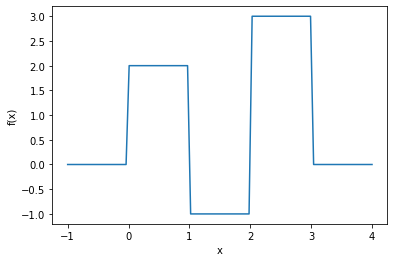
\includegraphics[width=10cm]{p1-2.png}
\end{figure}

式$g(x)$はシグモイド関数の和で表現されているので、上記の性質を合成した関数gを作成することができる。
ここで考えることは、ステップ関数の変換点と高さである。変換点として考えるべきなのは$x = 0,1,2,3$である。高さの変化については、$x=0:+2$、$x=1:-3$、$x=2:+4$、$x=3:-3$となっている。
高さについては、パラメータvの値を見ていくと、$x=0$において高さ$v_0 = 2$,$x=1$において高さ$v_1 = -2,v_2 = -1$,$x=2$において高さ$v_2 = 1,v_3 = 3$,$x=3$において高さ$v_6 = -3$のステップ関数をそれぞれ適用することで、$||f(x) - g(x)|| < \epsilon$となるようなパラメータbを決定することができる。

(本問題で作成したソースコードは\url{https://github.com/naoyaaan/AdvancedMachineLearning/blob/main/Okazaki/final.ipynb}にアップロードしています。)
\newpage
\section{問題2}

\subsection*{(1)}
\begin{equation*}
    h = 
    \begin{pmatrix}
        0 \\
        1.5
    \end{pmatrix}
\end{equation*}

\begin{equation*}
    \hat{y} = 0.5
\end{equation*}

\subsection*{(2)}

\begin{figure}[hbtp]
    \centering
    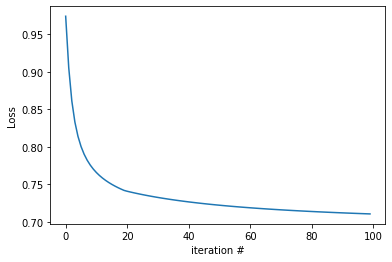
\includegraphics[width=10cm]{p2-1.png}
\end{figure}

\begin{figure}[hbtp]
    \centering
    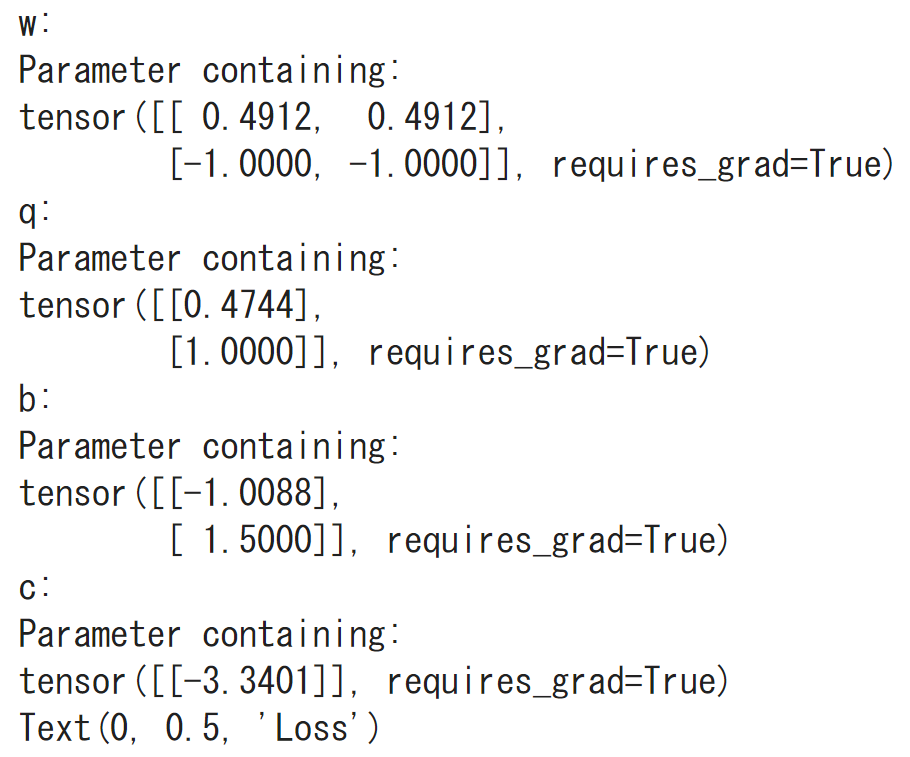
\includegraphics[width=9cm]{p2-2.png}
\end{figure}

(本問題で作成したソースコードは\url{https://github.com/naoyaaan/AdvancedMachineLearning/blob/main/Okazaki/final.ipynb}にアップロードしています。)

\newpage
\section{問題3}

\subsection{WordSim-353}
\subsubsection*{評価に用いられるタスクの概要}
\textbf{WordSim-353(WS353)}は単語の類似性または関連性を測るためのデータセットである。
Word Similarity Task(単語の類似性を測るタスク)では、モデルによる単語間の類似性の評価と人間による評価の相関を計測する。

\subsubsection*{データセットの統計情報}
データセットの統計情報は以下の表\cite{Recursive NN}のようである。

\begin{figure}[hbtp]
    \centering
    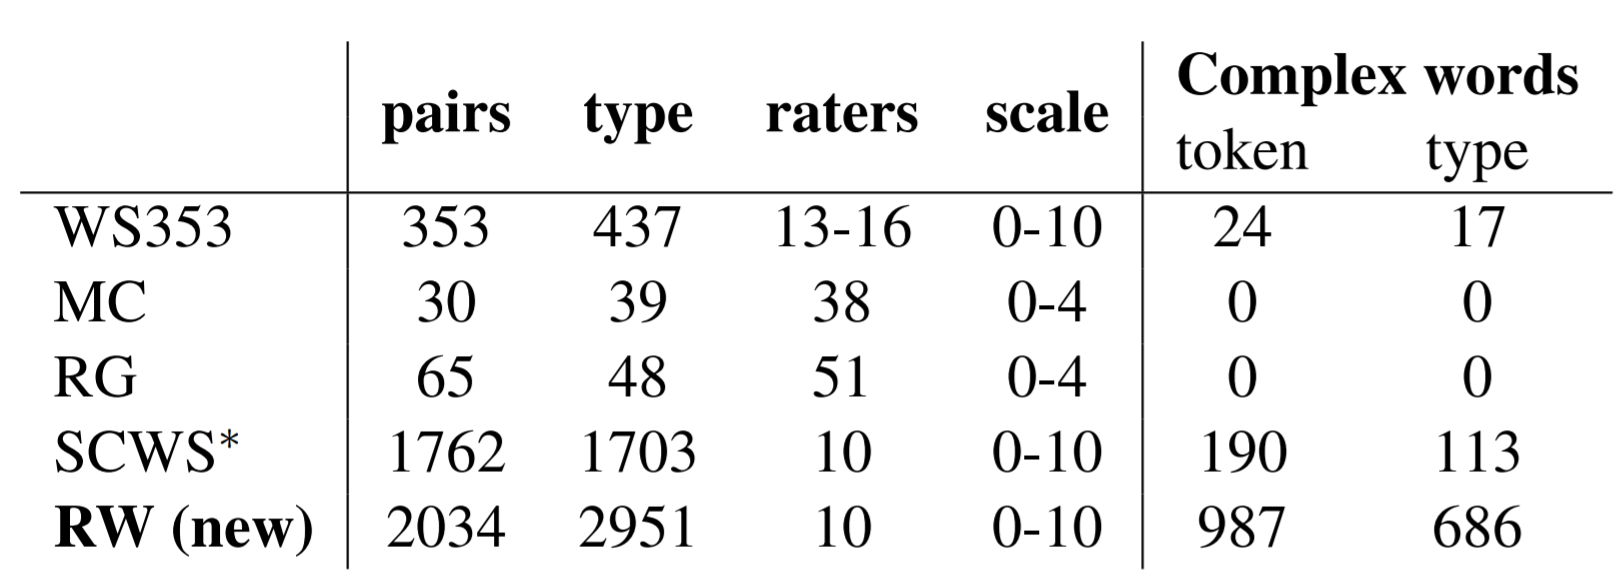
\includegraphics[width=10cm]{p3-1.png}
\end{figure}

pairsは類似性を測る二つの単語を、ratersは評価した人間の人数,scaleは類似性のスコアを表している。

\subsubsection*{評価の尺度}
上記のタスクによる評価には Spearman’s rank correlation coefficientの値($\rho$×100)が用いられる。
$\rho$は[-1,1]の値をとり、この値が大きいほど、人間の評価とモデルの評価に相関があることを表している。
以下の表\cite{fasttext}は実際にこのデータセットを用いてモデルを評価したときの結果である。

\begin{figure}[hbtp]
    \centering
    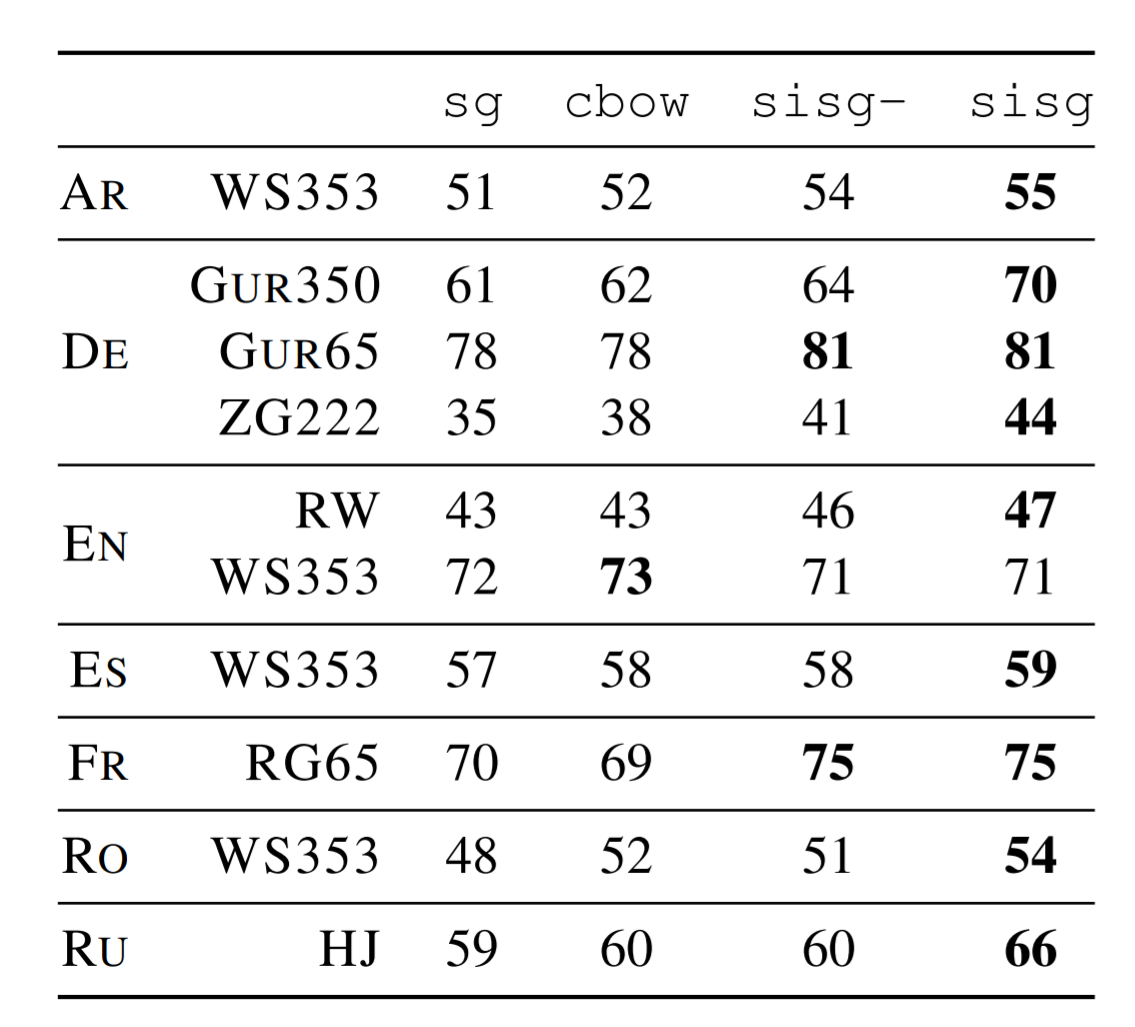
\includegraphics[width=10cm]{p3-2.png}
\end{figure}

\newpage
\subsection{IMDb}
\subsubsection*{評価に用いられるタスクの概要}
\textbf{IMDb}はテキスト分類のタスクを評価するために用いられる。具体的には、Sentiment Analysis, Topic Detection, Language Detectionなどのタスクがある。
Sentiment Analysisは、 テキストがポジティブかネガティブがどちらでもないかを測るタスクである。Topic Detectionは、自動的にそのテキスト、文章のテーマ、トピックを特定するタスクである。Language Detectionは、与えられたテキストの言語を決定するタスクである。

\subsubsection*{データセットの統計情報}
IMDbはthe Internete Movie Databaseというサイトにおける、ポジティブ、ネガティブをラベル付けされた50000件のレビューからなるデータセットである。
ポジティブとネガティブのレビューが同じ数だけ収録されている。10段階の評価で4以下がネガティブ、7以上がポジティブと判断している。

\subsubsection*{評価の尺度}
IMDbを用いたSentiment Analysisでは、モデルのポジティブorネガティブの正答率(\%)を用いて評価している。
以下の表\cite{NLP-progress}は、現在のIMDbにおけるモデルの予測精度のランキングである。
\begin{figure}[hbtp]
    \centering
    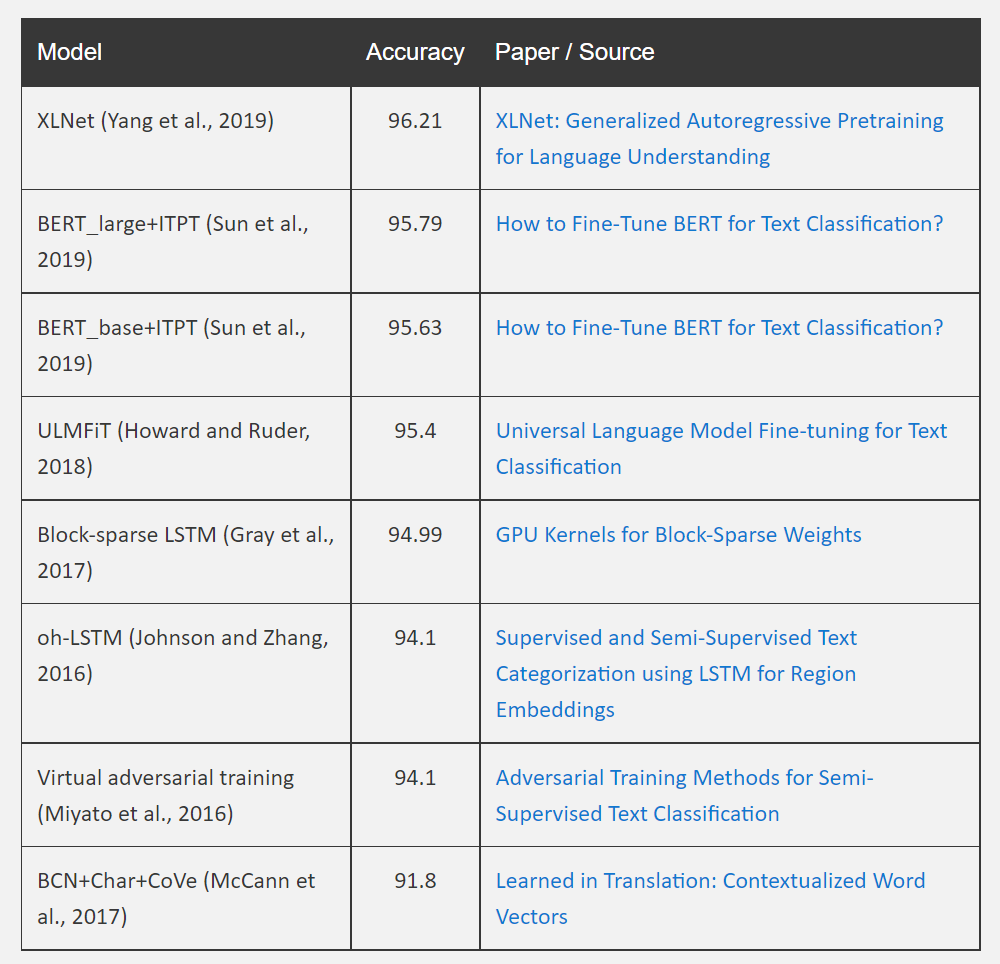
\includegraphics[width=10cm]{p3-3.png}
\end{figure}

\newpage
\section{問題4}
系列変換タスクにおいて、Transformerが再帰型ニューラルネットワーク(RNN)よりも優れている点として以下の2つが挙げられる。

1. 計算時間が早い

2. 並列化が可能

まずTransformerでは下図\cite{Attention}のような構造を用いている。

\begin{figure}[hbtp]
    \centering
    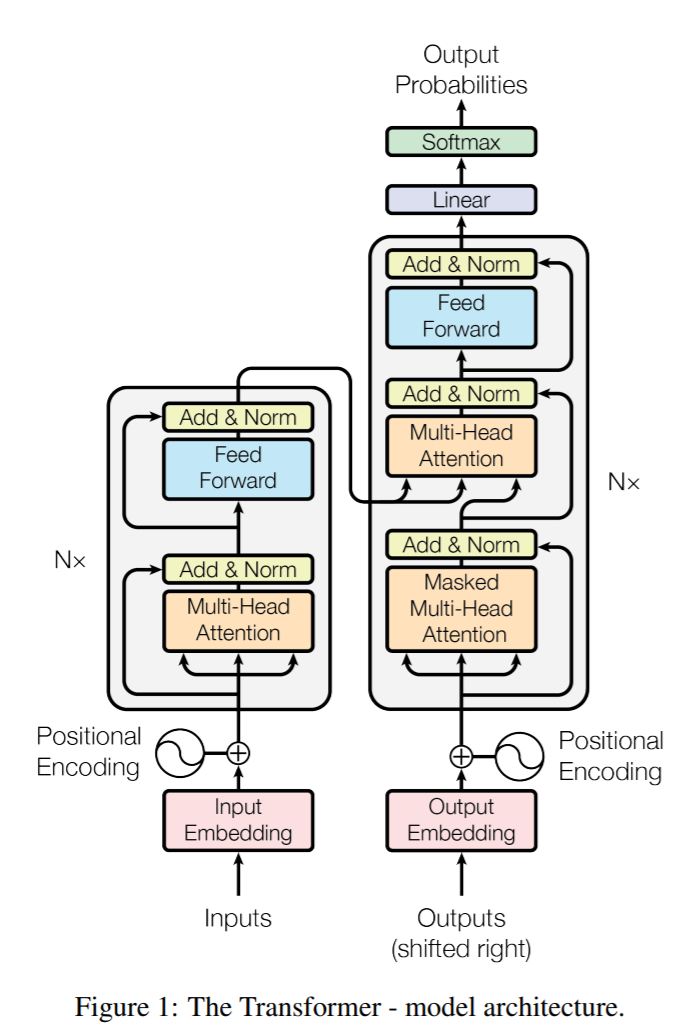
\includegraphics[width=5cm]{p4-2.png}
\end{figure}

この中でもTransformerにおいてはSelf-Attentionをベースとした構造となっている。
RNNをベースとした構造と比較したのが下表\cite{Attention}である。
\begin{figure}[hbtp]
    \centering
    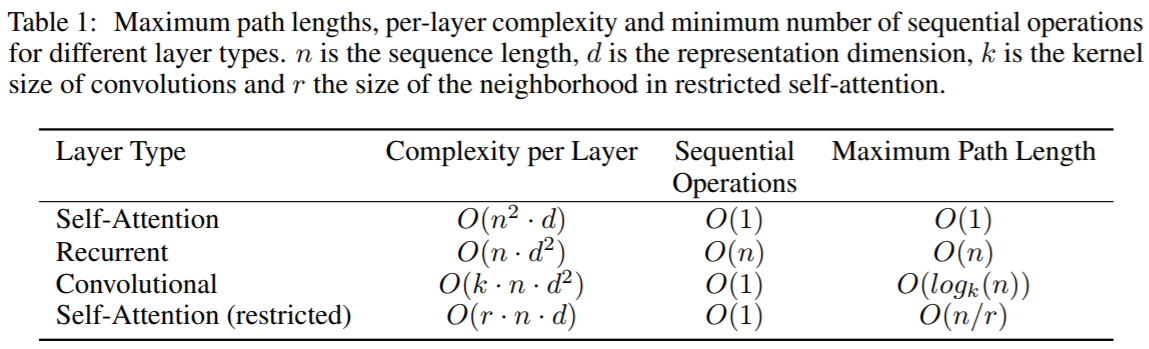
\includegraphics[width=12cm]{p4-1.png}
\end{figure}

これによると、RNNのレイヤーでは、$O(n^2\cdot d)$の計算量となっているが、Self-Attentionでは$O(n \cdot d^2)$となっている。
これだけではRNNがTransfomerより計算量が早いことはわからない。しかし、n(sequence length)やd(representation dimension)のサイズに注目してみると、たいていの場合$n < d$とnよりもdのほうがはるかに大きくなっている。そのため、Self-Attentionのレイヤーのほうが計算量が少ないことがわかる。

また、RNNでは入力に対してステップを経て処理をするので、Maximium path lengthの計算量は$O(n)$である。それにたいして、Self-Attentionは並列計算を行うので、Maximium path lengthの計算量は$O(1)$となっている。GPU演算を行うことを考えるとSelf-Attentionは並列化できることというのが計算量の削減につなっており、RNNの構造よりも優れた点であるといえる。


\newpage
\section{問題5}
\subsection*{この論文で検証したい仮説}
近年のTransformerのような自然言語処理システムでは、事前に学習された言語表現を用いる傾向がある。これらのモデルは文章読解や質問応答など多くの自然言語処理のタスクにおいて、充実した成果を挙げている。しかし、これらのモデルはタスクにとらわれない構造をしているものの、タスクに特化したデータセットとファインチューニングが必要である。これには、言語モデルの応用を制限してしまったり、ファインチューンによってきわめて限定的なタスク分布となってしまったり、人間であればほとんどの言語タスクを学習するためにたくさんの教師付きデータセットを必要としない、などの問題点がある。この論文では、データセットに特化した事前学習とファインチューニングを必要としないGPT-3のモデルで最新の研究を超えるような性能を発揮することを検証する。

\subsection*{その仮説を検証するための実験方法}
1750億のパラメーターを持つ自己回帰モデルのGPT-3を学習させ、文章学習能力を測ることで仮説を検証している。具体的には、20を超える自然言語処理のデータセットと、訓練データに直接含まれていないようなタスクへの高速な適応度をテストするために設計されたいくつかの重要なタスクにおいてGPT-3を評価している。各データセットにおいて、"few-shot learning"、"one-shot learning"、"zero-shot learning"の3つの状況において評価する。few,one,zeroはテストする際のデモンストレーションの数を表す。few-shot learningでは10-100のデモンストレーションを用いる。

\subsection*{GPT-3モデルのアーキテクチャ}
GPT-3ではGPT-2\cite{GPT-2}と同様のアーキテクチャを用いている。しかしGPT-3では、transformerにおいて、高密度でまとめられたスパースなアテンションが用いられている。

\subsection*{GPT-3モデルの学習に用いられたデータ}
下表\cite{GPT-3}に記載されているデータセットの集合を用いている。
\begin{figure}[hbtp]
    \centering
    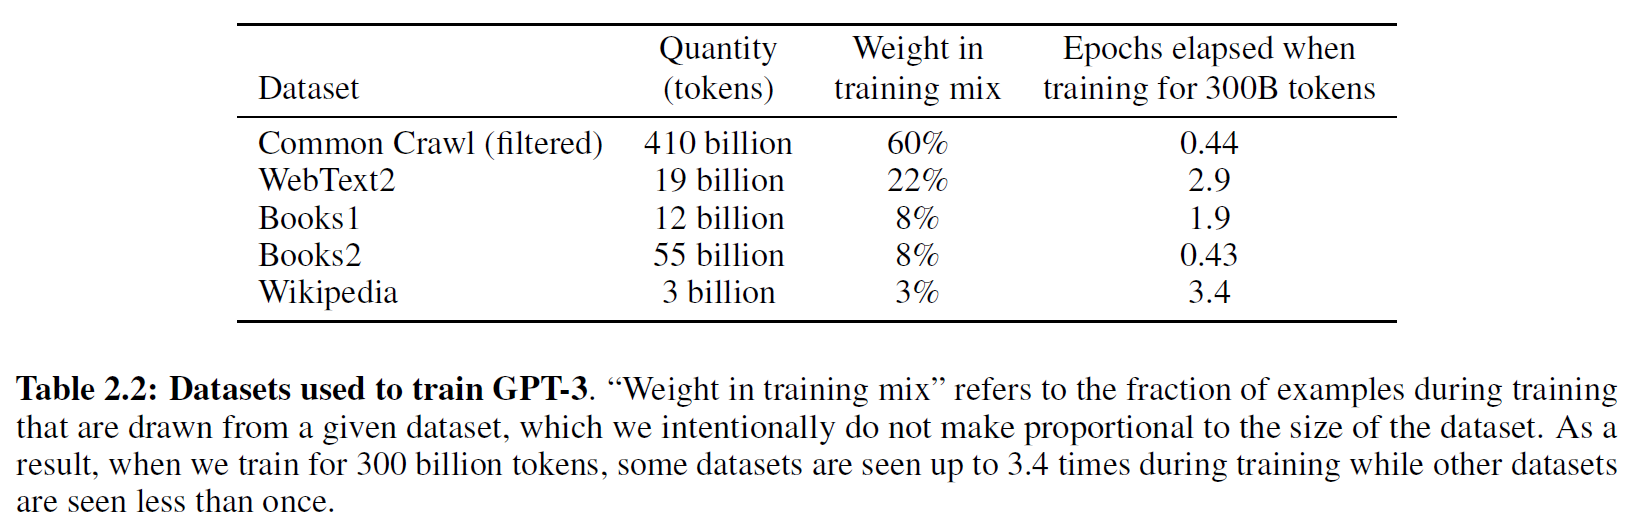
\includegraphics[width=15cm]{p5-1.png}
\end{figure}

\subsection*{実験に用いられたタスクやデータセットの概要}
以下に挙げるようなタスクやデータセットにおいて実験している。
traditional language modeling tasks, "closed book" question answering tasks, model's ability to translate betweeen language, Winogra Schema-like tasks, commonsense reasoning or question answering, reading comprehension tasks, SuperGLUE, NLI, additional tasks

\subsection*{実験結果の概要およびGPT-3で実現できたこと}
GPT-3では勾配の更新やアフィンチューニングなしに多くの自然言語処理のデータセットにおいて強力なパフォーマンスを達成した。zero-shot, one-shot learingでは有望な結果が得られ、few-shot learningでは大体のタスクにおいて最新研究と同等か、それ以上の結果を出している。

\subsection*{GPT-3モデルでも実現できなかったこと}
ANLIデータセットのような自然言語推論タスクや、RACEやQuACのような読解のデータセットにおいてはfew-shot learningは苦戦している。テキスト合成では意味的に同じことを繰り返すことがあるなどの問題があることがある。GPT-3には双方向性がないので双方向性が必要なタスクが少々困難、学習において重要度を考慮しておらず、効率が悪いこと、必要な容量が過多で不便であること、GPT-3の出力については解釈不能であることなどの問題点が残っている。

\newpage
\begin{thebibliography}{99}
    \bibitem{fasttext} Piotr Bojanowski, Edouard Grave, Armand Joulin, Tomas Mikolov. Enriching Word Vectors with Subword Information. arXiv:1607.04606. 2017
    \bibitem{Recursive NN} Minh-Thang, Luong Richard Socher, Christopher D. Manning. Better Word Representations with Recursive Neural Networks for Morphology.
    \bibitem{NLP-progress} NLP-progress. \url{http://nlpprogress.com/english/sentiment_analysis.html}. 閲覧日:2021年8月3日
    \bibitem{Attention} Ashish Vaswani, Noam Shazeer, Niki Parmar, Jakob Uszkoreit, Llion Jones, Aidan N. Gomez, Lukasz Kaiser, Illia Polosukhin. Attention Is All You Need. arXiv:1706.03762. 2017
    \bibitem{GPT-3} T. B. Brown, et al. Language Models are Few-Shot Learners. arXiv:2005.14165.
    2020.
    \bibitem{GPT-2} Alec Radford, Jeffrey Wu, Rewon Child, David Luan, Dario Amodei, and Ilya Sutskever. Language
    models are unsupervised multitask learners, 2019.

\end{thebibliography}

\end{document}